\documentclass[10pt, a5paper]{article}
\usepackage{pdfpages}
\usepackage{parallel}
\usepackage[T2A]{fontenc}
\usepackage{ucs}
\usepackage[utf8x]{inputenc}
\usepackage[polish,english,russian]{babel}
\usepackage{hyperref}
\usepackage{rotating}
\usepackage[inner=2cm,top=1.8cm,outer=2cm,bottom=2.3cm,nohead]{geometry}
\usepackage{listings}
\usepackage{graphicx}
\usepackage{wrapfig}
\usepackage{longtable}
\usepackage{indentfirst}
\usepackage{array}
\newcolumntype{P}[1]{>{\raggedright\arraybackslash}p{#1}}
\frenchspacing
\usepackage{fixltx2e} %text sub- and superscripts
\usepackage{icomma} % коскі ў матэматычным рэжыме
\PreloadUnicodePage{4}

\newcommand{\longpage}{\enlargethispage{\baselineskip}}
\newcommand{\shortpage}{\enlargethispage{-\baselineskip}}

\def\switchlang#1{\expandafter\csname switchlang#1\endcsname}
\def\switchlangbe{
\let\saverefname=\refname%
\def\refname{Літаратура}%
\def\figurename{Іл.}%
}
\def\switchlangen{
\let\saverefname=\refname%
\def\refname{References}%
\def\figurename{Fig.}%
}
\def\switchlangru{
\let\saverefname=\refname%
\let\savefigurename=\figurename%
\def\refname{Литература}%
\def\figurename{Рис.}%
}

\hyphenation{admi-ni-stra-tive}
\hyphenation{ex-pe-ri-ence}
\hyphenation{fle-xi-bi-li-ty}
\hyphenation{Py-thon}
\hyphenation{ma-the-ma-ti-cal}
\hyphenation{re-ported}
\hyphenation{imp-le-menta-tions}
\hyphenation{pro-vides}
\hyphenation{en-gi-neering}
\hyphenation{com-pa-ti-bi-li-ty}
\hyphenation{im-pos-sible}
\hyphenation{desk-top}
\hyphenation{elec-tro-nic}
\hyphenation{com-pa-ny}
\hyphenation{de-ve-lop-ment}
\hyphenation{de-ve-loping}
\hyphenation{de-ve-lop}
\hyphenation{da-ta-ba-se}
\hyphenation{plat-forms}
\hyphenation{or-ga-ni-za-tion}
\hyphenation{pro-gramming}
\hyphenation{in-stru-ments}
\hyphenation{Li-nux}
\hyphenation{sour-ce}
\hyphenation{en-vi-ron-ment}
\hyphenation{Te-le-pathy}
\hyphenation{Li-nux-ov-ka}
\hyphenation{Open-BSD}
\hyphenation{Free-BSD}
\hyphenation{men-ti-on-ed}
\hyphenation{app-li-ca-tion}

\def\progref!#1!{\texttt{#1}}
\renewcommand{\arraystretch}{2} %Іначай формулы ў матрыцы зліпаюцца з лініямі
\usepackage{array}

\def\interview #1 (#2), #3, #4, #5\par{

\section[#1, #3, #4]{#1 -- #3, #4}
\def\qname{LVEE}
\def\aname{#1}
\def\q ##1\par{{\noindent \bf \qname: ##1 }\par}
\def\a{{\noindent \bf \aname: } \def\qname{L}\def\aname{#2}}
}

\def\interview* #1 (#2), #3, #4, #5\par{

\section*{#1\\{\small\rm #3, #4. #5}}

\def\qname{LVEE}
\def\aname{#1}
\def\q ##1\par{{\noindent \bf \qname: ##1 }\par}
\def\a{{\noindent \bf \aname: } \def\qname{L}\def\aname{#2}}
}

\switchlang{ru}
\begin{document}
\title{Разработка архитектуры Game-stream платформы на основе OpenSource компонентов\footnote{\url{arol90@gmail.com}, \url{https://lvee.org/en/abstracts/276}}}
\author{Антон Новиков, Минск, Belarus}
\maketitle
\begin{abstract}
A game stream service development and architecture specifics are covered with focus on the open source components. Personal experience of building such service is covered, including compo\-nents choice and resulting performance.
\end{abstract}
\section*{Введение}

В настоящее время активно развивается направление games as a service. Основной задачей таких сервисов является предоставление возможности потребителю быстро и, главное, не имея достаточных вычислительных ресурсов, получить игровой опыт неотличимый от запуска игры на своем компьютере.

Подобные сервисы существуют достаточно давно, но зачастую являются проприетарными и недоступными для использования иначе чем в потребительских целях на платной основе.

%%\begin{center}
%%\begin{figure}[h!]
%%  \centering
%%  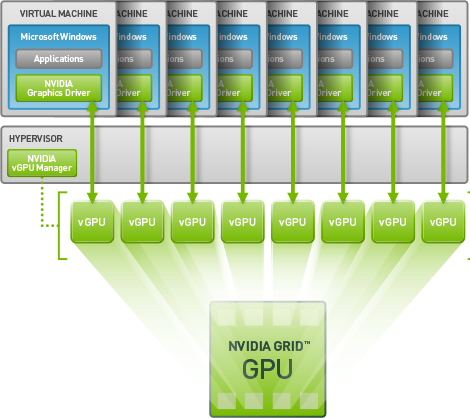
\includegraphics[width=5.5cm]{11_2018_Novikov1}
%%%  \caption{~}
%%%  \label{fig:Kharkevich1}
%%\end{figure}
%%\end{center} 

Главной предпосылкой появления возможности трансляции игр в виде видео-потока на компьютер пользователя стало появление в системах виртуализации технологии проброса графического адаптера (либо части графического адаптера) в виртуальную машину. Эта технология обширно используется в профессиональной среде с CAD-приложениями, давая возможность разделения одного мощного графического адаптера на несколько потребителей.

Также существуют и другие возможности применения данной схемы – например, математическое расчеты на GPU, построение 3D-моделей, рендеринг видео и другие.

Разрабатываемая автором по данной схеме система потокового game-сервиса является универсальной и полнофункциональной. Её особенности раскрыты ниже.

\section*{Архитектура}

Архитектура подобного рода сервисов зачастую является <<конструктором>> из множества различных по функциональному назначению модулей и компонентов:
\begin{itemize}
\item аппаратная платформа;
\item ОС для аппаратной платформы;
\item ОС для виртуальных машин;
\item средства управления и оркестрации;
\item средства кластеризации и распределения нагрузок;
\item приложения.
\end{itemize}

\section*{Front-end и биллинг}

В качестве опорных точек были выбраны некоторые основные аспекты:
\begin{itemize}
\item Каждое приложение~--- это отдельная виртуальная машина.
\item Все функции по обслуживанию виртуальных машин берёт на себя система виртуализации.
\item ОС для запуска приложения должна быть стабильным LTS-дистрибутивом GNU/Linux.
\item Система виртуализации имеет функционал частичного проброса графического адаптера.
\item Возможность использования как на физических серверах в собственном ЦОД, так и на арендованных выделенных серверах облачных провайдеров.
\end{itemize}
\section*{Обоснование выбора компонентов}

\subsection*{Аппаратная платформа} 
В зависимости от сложности приложений необходимо учитывать вычислительные мощности; поэтому было разработано несколько концепций вычислительного сервера и его усредненная модель:
\begin{itemize}
\item 2 CPU Intel Xeon 8 core 2.66 ГГц; 
\item 128 GB RAM;
\item 4 карты Nvidia Tesla P100;
\item корпус с возможностью установки графических карт.
\end{itemize}

\subsection*{ОС для аппаратной платформы}
Выбор системы виртуализации первоочередно обоснован возможностью проброса графического адаптера в ВМ, и самой продвинутой по этой части из свободных платформ на данный момент является XCP-next generation (основанный на базе XEN Server, под лицензией GNU General Public License). Также и все библиотеки Nvidia, необходимые для осуществления требуемого функционала, распространяются на свободной основе.

Система имеет возможности частичного и полного проброса, встроенные средства управления кластером, мониторинга, резервного копирования и полностью совместима с гипервизором, используемым в AWS, что дает возможность развертывания платформы в арендованных облаках.

В дополнение к функционалу гипервизора была добавлена система оркестрации XenOrchestra (также под свободной лицензией, AGPLv3).

\subsection*{ОС для виртуальных машин}
Для запуска большинства игр из библиотеки Steam, которые совместимы с ОС Linux, необходима Debian-подобная система (Steam OS). Именно стабильная версия ОС Debian 9 легла в основу золотого образа. Также могли бы быть использованы и другие ОС: SteamOS в режиме киоска, Ubuntu 16.04 LTS для разработки и создания игр на графическом движке Unreal Engine 4.

Во всей архитектуре использована концепция <<одна игра = одна виртуальная машина>>, такой подход позволяет легко клонировать и перемещать игры внутри вычислительного кластера, разделять ресурсы, и быстро запускать игры по запросу пользователя.

\subsection*{Front-end и биллинг} 
В отношении клиентской части перед командой разработчиков стояла задача разработки системы биллинга и конечного клиентского приложения, но существует возможность использования и готовых решений.
\subsection*{Стрим-приложения}
Непосредственно захват изображения, рендеринг, кодирование его для передачи производились на графическом адаптере. Новые поколения графических карт имеют возможность одновременной работы как рендерера, так и энкодера – при помощи всего лишь стандартного функционала. Для программной обработки были использованы свободные библиотеки OpenBroadcasterSoftware (GNU General Public License, version 2) и стандартный функционал приложения.

\section*{Сравнение производительности}
При развёртывании стенда для тестирования производительности полученной системы и сравнения её с аналогами были использованы также готовые виртуальные машины на AWS, основанные на Windows 2016 Server. Результаты тестирования отличались на уровне погрешности, но следует заметить, что платформа, основанная на свободном ПО, отличается большей гибкостью и возможностями применения, проприетарная же платформа ограничена играми. Если использовать платформу только для игр, то платформа на основе Windows находится в преимуществе исключительно из-за количества доступных игр.

\section*{Заключение}
Разработанная архитектура прошла все этапы тестирования и успешно используется для различных целей, легко адаптируемая под задачи: Разработка игр, стрим игр, обработка 3d графики, CAD приложения, ДЕМО 3d приложения, вычисления с использованием GPU. 
Легкость адаптации, бесконечное горизонтальное масштабирование, возможность использоваться на арендованных облаках и гибридных облаках делают систему универсальной платформой и мощным инструментом собранным исключительно из свободных компонентов.

\end{document}
